\documentclass{beamer}




\usepackage[T1,T2A]{fontenc}
\usepackage[utf8]{inputenc}

\usepackage{graphicx}
\usepackage{blindtext}
\usepackage{ mathrsfs }
\usepackage[russian,english]{babel}

\author{Деркач Максим Юрьевич}
\title{Криптографические протоколы}
\subtitle{Лекция 4 \\ Протоколы аутентификации: классификация, атаки \\ Протоколы "слабой" аутентификации }


%\usetheme{lucid}
\begin{document}
	\frame {
		\titlepage
	}
	\frame {
		\frametitle{Ссылки}
		
		\url{https://habr.com/post/154229/}
		\url{https://habr.com/en/company/dataart/blog/262817/}
		\url{https://en.wikipedia.org/wiki/Pass_the_hash}
		
	}
	\frame {
		\frametitle{Протоколы аутентификации}
		\framesubtitle{Определения}
		
		\textbf{Определение 1}
		
		\textbf{Аутентификация} - подтверждение подлинности.
		
		\bigskip
		\textbf{Определение 2}
		
		\textbf{Идентификация} - однозначное именование (присвоение уникальных имён или признаков) компонентов
								автоматизированной системы и всех лиц (пользователей), взаимодействующих с системой. 
		
		\bigskip
		\textbf{Определение 3}
		
		\textbf{Протокол аутентификации} - криптографический протокол, в ходе которого одна сторона	удостоверяется в
								идентичности другой стороны, вовлеченной в протокол, а также убеждается в том, что
								вторая сторона активна во время или непосредственно	перед моментом выполнения протокола.   
		\bigskip
	}
	\frame{
		\frametitle{Классификация аутентификации}
		\begin{itemize}
			\item[+] По количеству доказывающих сторон:
				\begin{itemize}
							\item[*] одностороняя - доказывающая сторона $A$  и проверяющая сторона $B$;
							\item[*] двустороняя - обе стороны $A$  и $B$ доказывают свою подлинность друг другу.
				\end{itemize}
			
			\bigskip
			
			\item[+] По устойчивости:
			\begin{itemize}
				\item[*] протоколы "слабой" аутентификации (на основе фиксированных или одноразовых паролей);
				\item[*] протоколы "сильной" аутентификации (на основе запроса типа "вопрос-ответ");
				\item[*] протоколы основанные на техники доказательства знания.
			\end{itemize}
			
		\end{itemize}
	
		\bigskip
		
		Цель протокола - установление того факта, что проверяемая сторона является той, за кого она себя выдаёт.
		
		\bigskip
		
		Возможны два исхода: подтверждение подлинности, не подтверждение.	
	}

	\frame{
		\frametitle{Протоколы слабой аутентификации}
		\framesubtitle{Фиксированные пароли}
		
		\bigskip
		
		$A -> S: ID_A || P$
		
		\bigskip
		
		\textbf{Угрозы:}
		\begin{enumerate}
			\item раскрытие пароля (разглашение, восстановление из системной информации);
			\item перехват пароля (внутри системы);
			\item угадывание пароля.
		\end{enumerate}
	
		\bigskip
		
		\textbf{Атаки на фиксированные пароли:}
		\begin{enumerate}
			\item повторное использование пароля;
			\item тотальный перебор;
			\item атака со словарём.
		\end{enumerate}
		
	}
	
	\frame{
		\frametitle{Фиксированные пароли}
		\framesubtitle{Приёмы повышения стойкости}
		
	
		\begin{enumerate}
			\item Хранение в компьютерной системе файлов паролей в защищенном режиме 
					(с защитой от чтения/записи).
			\item Xранение в системе не	самих паролей, а их	образов. 
			\item Задание правил выбора	паролей.
			
			\item Ограничение попыток ввода пароля.
			\item Добавление "соли" к паролю (добавление случайной величины	к паролю
					перед обработкой его однонаправленной функцией).
			\item Многофакторная аутентификация. 
		\end{enumerate}	
		
	}

		\frame{
		\frametitle{Фиксированные пароли}
		\framesubtitle{Многофакторная аутентификация}
		
		
		\begin{enumerate}
			\item Смарт-карта
			\item Электронный идентификатор
			\item Биометрические аутентификаторы
			\item SMS-аутентификация
		\end{enumerate}	
		
	}
	
	\frame{
		\frametitle{Фиксированные пароли}
		\framesubtitle{Использование криптографических методов для повышения стойкости}
		
		\bigskip
		
		 На сервере обычно хранятся пароли в зашифрованном виде либо хэш от пароля.
		
		\bigskip
		\begin{enumerate}
			\item $A -> S: ID_A$
			\item $S -> A: R_S || text_A$
			\item $A -> S: ID_A || h_1(R_S || h_2(p_A || text_A))$
		\end{enumerate}	
		
		\bigskip
		
		где $ID_A, text_A, h_2(p_A || text_A)$ хранятся на проверяющей стороне(сервере).
		
		\bigskip
		
		Однако такой протокол неустойчив к атаке MITM и атаке параллельного сеанса.
	}

\frame{
	\frametitle{Фиксированные пароли [Примеры]}
	\framesubtitle{HTTP authentication}
	
	\bigskip
	
	Этот протокол, описанный в стандартах HTTP 1.0/1.1, существует 	очень давно и до сих пор активно применяется в корпоративной среде. Применительно к веб-сайтам работает следующим образом:

	\bigskip
	\begin{enumerate}
		\item Сервер, при обращении неавторизованного клиента к защищенному ресурсу, отсылает HTTP статус “401 Unauthorized” и добавляет заголовок “WWW-Authenticate” с указанием схемы и параметров аутентификации.

		\item Браузер, при получении такого ответа, автоматически показывает диалог ввода username и password. Пользователь вводит детали своей учетной записи.

		\item Во всех последующих запросах к этому веб-сайту браузер автоматически добавляет HTTP заголовок “Authorization”.

		\item Сервер аутентифицирует пользователя по данным из этого заголовка. 

	\end{enumerate}	
	}

	\frame{
	\frametitle{Фиксированные пароли [Примеры]}
	\framesubtitle{HTTP authentication[Basic]}
	
	\bigskip
	
	\textbf{Basic} — наиболее простая схема, при которой username и password пользователя передаются в заголовке Authorization в незашифрованном виде (base64-encoded). Однако при использовании HTTPS (HTTP over SSL) протокола, является относительно безопасной.
	
	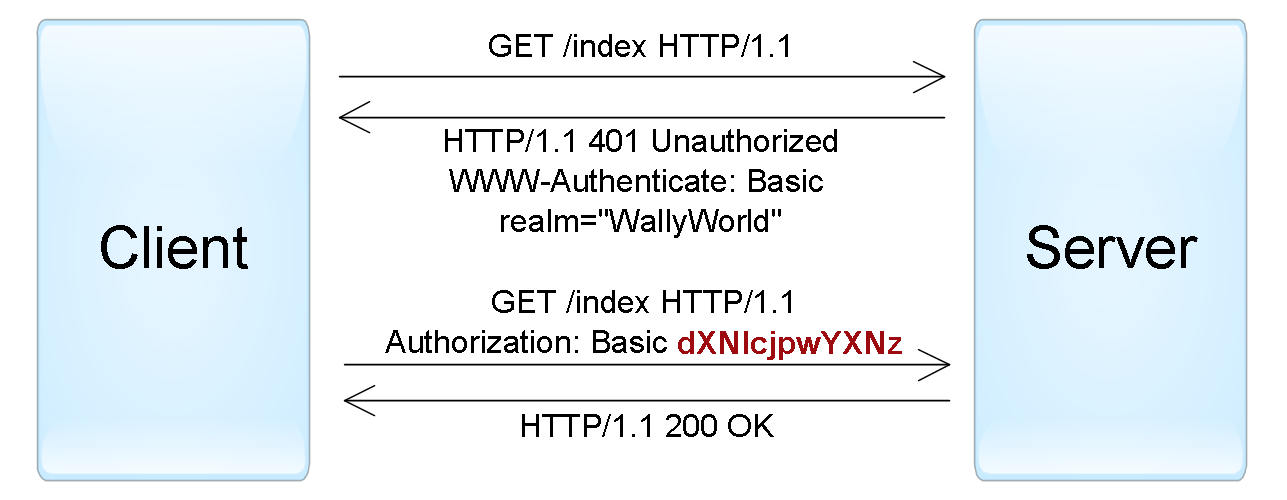
\includegraphics[width=0.8\linewidth]{basic_auth.png}
	
	}

	\frame{
	\frametitle{Фиксированные пароли [Примеры]}
	\framesubtitle{HTTP authentication[Digest]}
	
	\bigskip
	
	\textbf{Digest} — challenge-response-схема, при которой сервер посылает уникальное значение nonce, а браузер передает MD5 хэш пароля пользователя, вычисленный с использованием указанного nonce. Более безопасная альтернативв Basic схемы при незащищенных соединениях, но подвержена man-in-the-middle attacks.
	
	}

	\frame{
		\frametitle{Фиксированные пароли [Примеры]}
		\framesubtitle{HTTP authentication[NTLM, Negotiate]}
		
		\bigskip
		
		\textbf{NTLM} —  также основана на challenge-response подходе, при котором пароль не передается в чистом виде. Эта схема не является стандартом HTTP, но поддерживается большинством браузеров и веб-серверов. Преимущественно используется для аутентификации пользователей Windows Active Directory в веб-приложениях. Уязвима к pass-the-hash-атакам.
		
		\bigskip
		
		\textbf{Negotiate} - ще одна схема из семейства Windows authentication, которая позволяет клиенту выбрать между NTLM и Kerberos аутентификацией.
		
		\bigskip
		
		Стоит отметить, что при использовании HTTP-аутентификации у пользователя нет стандартной возможности выйти из веб-приложения, кроме как закрыть все окна браузера.
		
	}

	\frame{
		\frametitle{Фиксированные пароли [Примеры]}
		\framesubtitle{Другие протоколы аутентификации по паролю}
		
		\begin{enumerate}
			\item \textbf{Forms authentication} - наиболее популярный метод аутентификации.
			
			\item \textbf{URL query} — считается небезопасным вариантом, т. к. строки URL могут запоминаться браузерами, прокси и веб-серверами.
			
			\item \textbf{HTTP header} — оптимальный вариант, при этом могут использоваться и стандартный заголовок Authorization (например, с Basic-схемой), и другие произвольные заголовки.
			
		\end{enumerate}
	}

		\frame{
		\frametitle{Фиксированные пароли [Примеры]}
		\framesubtitle{Распространенные уязвимости и ошибки реализации}
		
		\begin{enumerate}
			\item Веб-приложение позволяет пользователям создавать простые пароли.
			
			\item Веб-приложение не защищено от возможности перебора паролей (brute-force attacks).
			
			\item Веб-приложение само генерирует и распространяет пароли пользователям, однако не требует смены пароля после первого входа (т.е. текущий пароль где-то записан).
			
			\item Веб-приложение допускает передачу паролей по незащищенному HTTP-соединению, либо в строке URL.
			
			\item Веб-приложение не использует безопасные хэш-функции для хранения паролей пользователей.
			
			
		\end{enumerate}
	}

	\frame{
	\frametitle{Фиксированные пароли [Примеры]}
	\framesubtitle{Распространенные уязвимости и ошибки реализации}
		
		\begin{enumerate}
			\setcounter{enumi}{5}
			\item Веб-приложение использует уязвимую функцию восстановления пароля, которую можно использовать для получения несанкционированного доступа к другим учетным записям.
			
			\item  Веб-приложение не требует повторной аутентификации пользователя для важных действий: смена пароля, изменения адреса доставки товаров и т. п.
			
			\item Веб-приложение создает session tokens таким образом, что они могут быть подобраны или предсказаны для других пользователей.
			
			\item Веб-приложение допускает передачу session tokens по незащищенному HTTP-соединению, либо в строке URL.
			
		\end{enumerate}
	}

	\frame{
	\frametitle{Фиксированные пароли [Примеры]}
	\framesubtitle{Распространенные уязвимости и ошибки реализации}
	
	\begin{enumerate}
			\setcounter{enumi}{9}
		\item Веб-приложение не предоставляет пользователям возможность изменения пароля либо не нотифицирует пользователей об изменении их паролей.

		\item Веб-приложение уязвимо для session fixation-атак (т. е. не заменяет session token при переходе анонимной сессии пользователя в аутентифицированную).
		
		\item Веб-приложение не устанавливает флаги HttpOnly и Secure для browser cookies, содержащих session tokens.
		
		\item Веб-приложение не уничтожает сессии пользователя после короткого периода неактивности либо не предоставляет функцию выхода из аутентифицированной сессии.
		
	\end{enumerate}
}

	\frame{
	\frametitle{Одноразовые пароли}
		\begin{enumerate}
			\item Разделяемые списки одноразовых паролей:
				пользователь и система имеют заранее определенный список паролей, который каждый из них хранит самостоятельно. 
				При выполнении очередного сеанса протокола аутентификации выбирается пользователем и проверяется системой очередной пароль из этого списка .
									
			\item Последовательно обновляемые одноразовые пароли:
				Первоначально пользователь и система имеют только один пароль ,  условно с номером i. Затем пользователь создает и передает системе пароль под номером i-1,
				зашифрованный на ключе, вычисленном из i-го пароля.  Такой метод затруднительно реализовать при ненадежном канале связи (при возможности обрыва связи).  
				
			\item Последовательности одноразовых паролей, основанные на	однонаправленных функциях.
			
		\end{enumerate}
	}

	\frame{
	\frametitle{Одноразовые пароли}
	\framesubtitle{Схема Лэмпорта с одноразовыми паролями \\ (RFC 1760 - The S/Key One-Time Password System)}
	
	На проверяющей стороне(сервере) хранятся $ID_A, h^n(p_A)$, где $n$ - достаточно большое.
	
	\bigskip
	\begin{enumerate}
		\item $A -> S: ID_A || h ^ {n - 1} (p_A)$
		\item Сервер вычисляет $h(h ^ {n - 1} (p_A))$ и сравнивает с хранящимися данными, если совпало, то аутентификация пройдена успешна,
		и запись обоновляется на $ID_A || h ^ {n - 1} (p_A)$.
	\end{enumerate}
	

	\bigskip
	\textbf{S/Key}
	\begin{enumerate}
		\item $A -> S: ID_A$
		\item $S -> A: m$
		\item $A -> S: h ^ {m - 1} (p_A)$
	\end{enumerate}	

	}

	\frame{
	\frametitle{Одноразовые пароли}
	\framesubtitle{Схема Лэмпорта с одноразовыми паролями \\ (RFC 1760 - The S/Key One-Time Password System)}
	
	\bigskip
	\textbf{Существует атака}
	\begin{enumerate}
		\item $A -> I(S): ID_A$
		\item $I(A) -> S: ID_A$
		
		\item $S -> I(A): m$
		\item $I(S) -> A: m - 1$
		
		\item $A -> I(S): h ^ {m - 2} (p_A)$
		\item $I(A) -> S: h(h ^ {m - 2} (p_A))$
		
	\end{enumerate}	
	
	\bigskip
	\textbf{Следующий раз}
	\begin{enumerate}
		\item $I(A) -> S: ID_A$
	
		\item $S -> I(A): m - 1$
		
		\item $I(A) -> S: h ^ {m - 2} (p_A)$
	
	\end{enumerate}	
	}
	
	\frame {
	\begin{figure}
		
\includegraphics[width=0.8\linewidth]{index1.jpeg}
	\end{figure}
	}

\end{document}